\clearpage
\section{Results and interpretation}

At the time of writing this thesis, the search presented here is in final stages of approval by a committee at CERN. Therefore, instead of unblinding the full run 2 luminosity, 10\% of the luminosity is unblinded in the following section. The results section will be divided into two parts. Section~\ref{sec:expected-limits} presents the expected limits of the full run 2 luminosity without observed data, which allows for comparison of the sensitivity of this search to previous searches. Section~{sec:unblinded-limits} presents the observed and predicted counts for the 10\% run 2 luminosity alongside the calculated limits. 

The results are interprted in terms of the compressed Higgsino simplified model described in Section~\ref{sec:search-introduction}. The calculation of both expected and observed limits has been done using the Higgs combination tool~\cite{higgs-combine-site}. It uses the standard CL${}_s$ technique~\cite{Junk:1999kv,A_L_Read_2002} to compute the limits at the 95\% Confidence Level (CL).

The limits are shown in the plane of $\dmpm-m_\PSGcpmDo$. As described in Section~\ref{sec:search-introduction}, $\dmo=2\dmpm$. The area inside the curves is excluded, while color-coded z axis shows the upper limit on the cross section. The green line shows the minimum $\dmpm$ allowed by the theoretical calculation which takes into account radiative corrections, as described in~\cite{Nagata_2015}.

\subsection{Expected limits for run 2}
\label{sec:expected-limits}

The expected limits for full run 2 luminosity are shown in Figure~\ref{fig:expected_limits}. The top row shows the exclusive track plus lepton categories, with the electron on the left and the muon on the right. As can be seen, these categories do not have exclusive power on their own, but rather they set upper limits on the cross section. They slightly improve the expected limits set by the dimuon category when combined with it, as can be seen by comparing the two plots in the middle row.

The plot on the left in the middle row shows the limit the expected limits set by the dimuon category, while the plot on the right shows the combination of the three categories. As can be seen, near the LEP limits, $\dmpm$ ($\dmo$) down to $0.8\GeV$ ($1.6\GeV$) is expected to be excluded. At higher mass splittings between 2 and $2.5\GeV$, chargino mass of up to almost $160\GeV$ is expected to be excluded. As can be seen, this analysis is expected to exclude mass splitting bellow the previous exclusion limits set at CMS in the SOS analysis.

The last plot in the bottom line shows the expected exclusion limits when the SOS orthogonality requirement is relaxed. It shows the potential of the analysis without the constraints of orthogonality. As can be seen, while it does not help in the very compressed region of around $1\GeV$, it does push the expected limit in the less compressed region to exclude chargino with a mass of above $170\GeV$.

\begin{figure}[!htb]
\centering
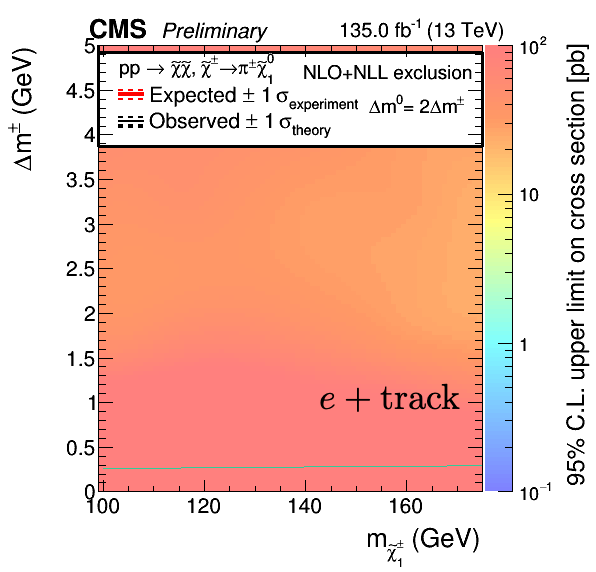
\includegraphics[width=0.48\linewidth]{plots/limits/expected/PureHiggsino_1tElectrons_ExpectedXSEC.png} \,
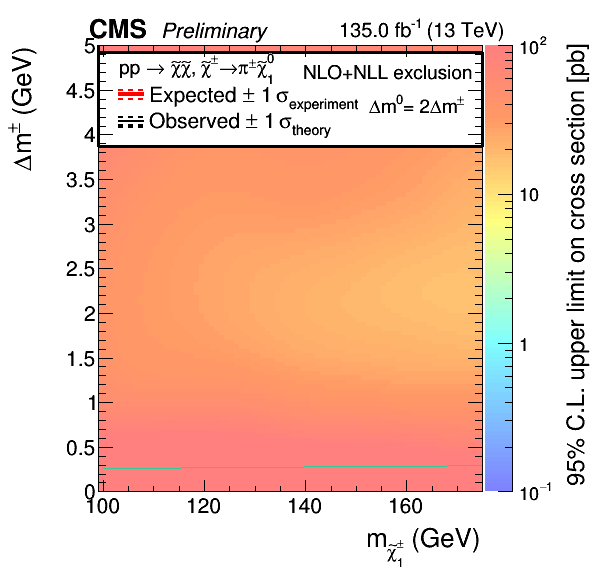
\includegraphics[width=0.48\linewidth]{plots/limits/expected/PureHiggsino_1tMuons_comb_ExpectedXSEC.png} \\

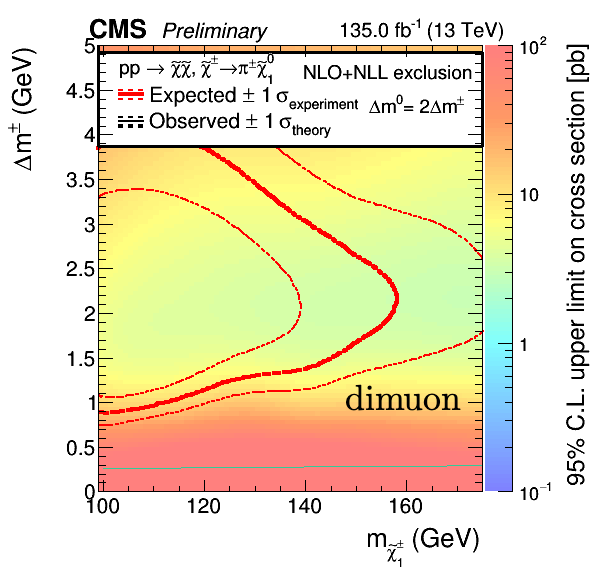
\includegraphics[width=0.48\linewidth]{plots/limits/expected/PureHiggsino_2lMuonsOrth_ExpectedXSEC.png} \,
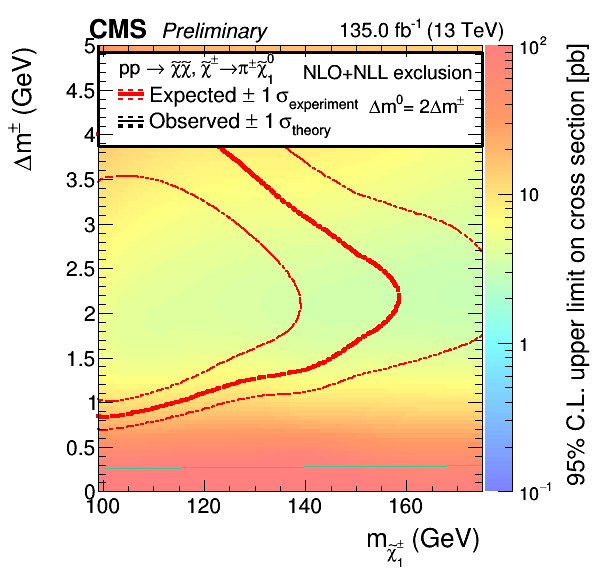
\includegraphics[width=0.48\linewidth]{plots/limits/expected/PureHiggsino_SoftPromptRun2_ExpectedXSEC.png} \\

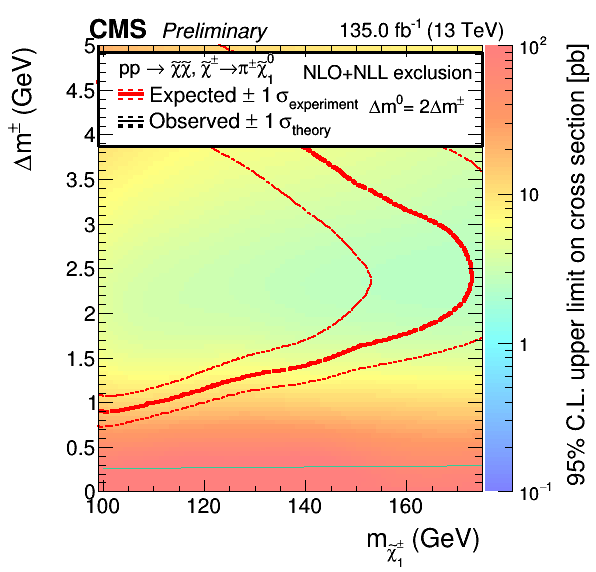
\includegraphics[width=0.48\linewidth]{plots/limits/expected/PureHiggsino_SoftPromptRun2Inc_ExpectedXSEC.png} \\

\caption[Expected limits for full run 2 luminosity]{Expected limits for full run 2 luminosity. Top row shows limits for exclusive track plus electron (muon) on the left (right). The middle row shows limits for the dimuon category (left) and the combined limits for all categories (right). The bottom row shows the combined limits for all categories for the relaxed condition without SOS orthogonality.}
\label{fig:expected_limits}
\end{figure}

\subsection{Partially unblinded results}
\label{sec:unblinded-limits}

In order to perform the unblinding of 10\% of the data, the background estimation which is data-driven uses the full run 2 luminosity scaled down by 0.1, while the data is taken 1 out of every 10 events. The data and background predictions are shown in Figure~\ref{fig:unblinded_results}. The results are shown for the muon plus track category in the first row, electron plus track category in the middle row, and the dimuon category in the bottom row. The largest excess is observed in the right-most bin of the dimuon category in phase 0. That excess corresponds to $1.4\sigma$, and is interpreted as agreeing with the SM. 

Since the results suggest no deviation from the SM, observed and expecte limits are produced in Figure~\ref{fig:observed_limits}. As expected, the much reduced luminosity approved for unblinding has reduced much the expected exclusion. In addition, due to the small excess observed in data in comparison with the expected count, no observed limit was able to be set.

\begin{figure}[!htb]
\centering
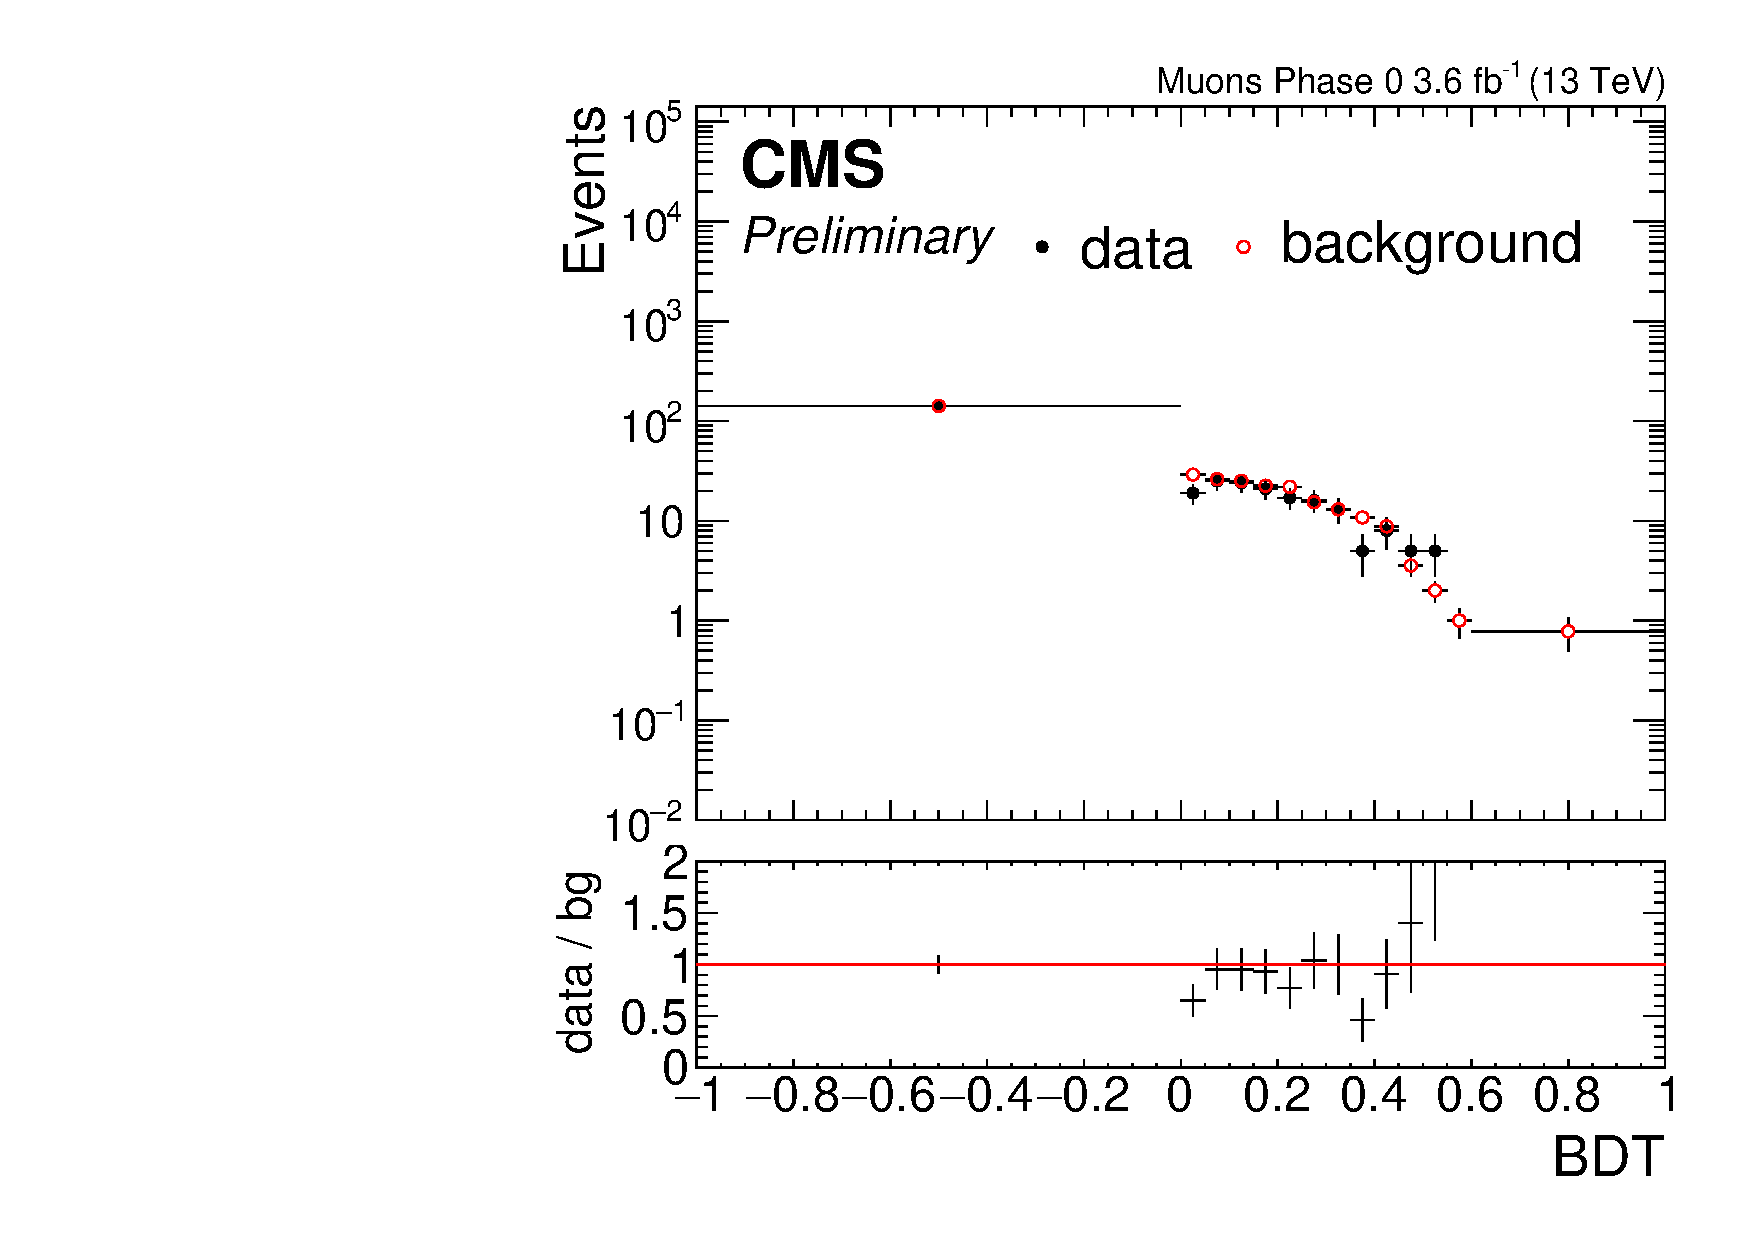
\includegraphics[width=0.48\linewidth]{plots/partial_unblinded_track_muon_sc_comparison/none_exTrack_dilepBDT_binsCorrJetNoMultIso10Dr0.6_log.pdf} \,
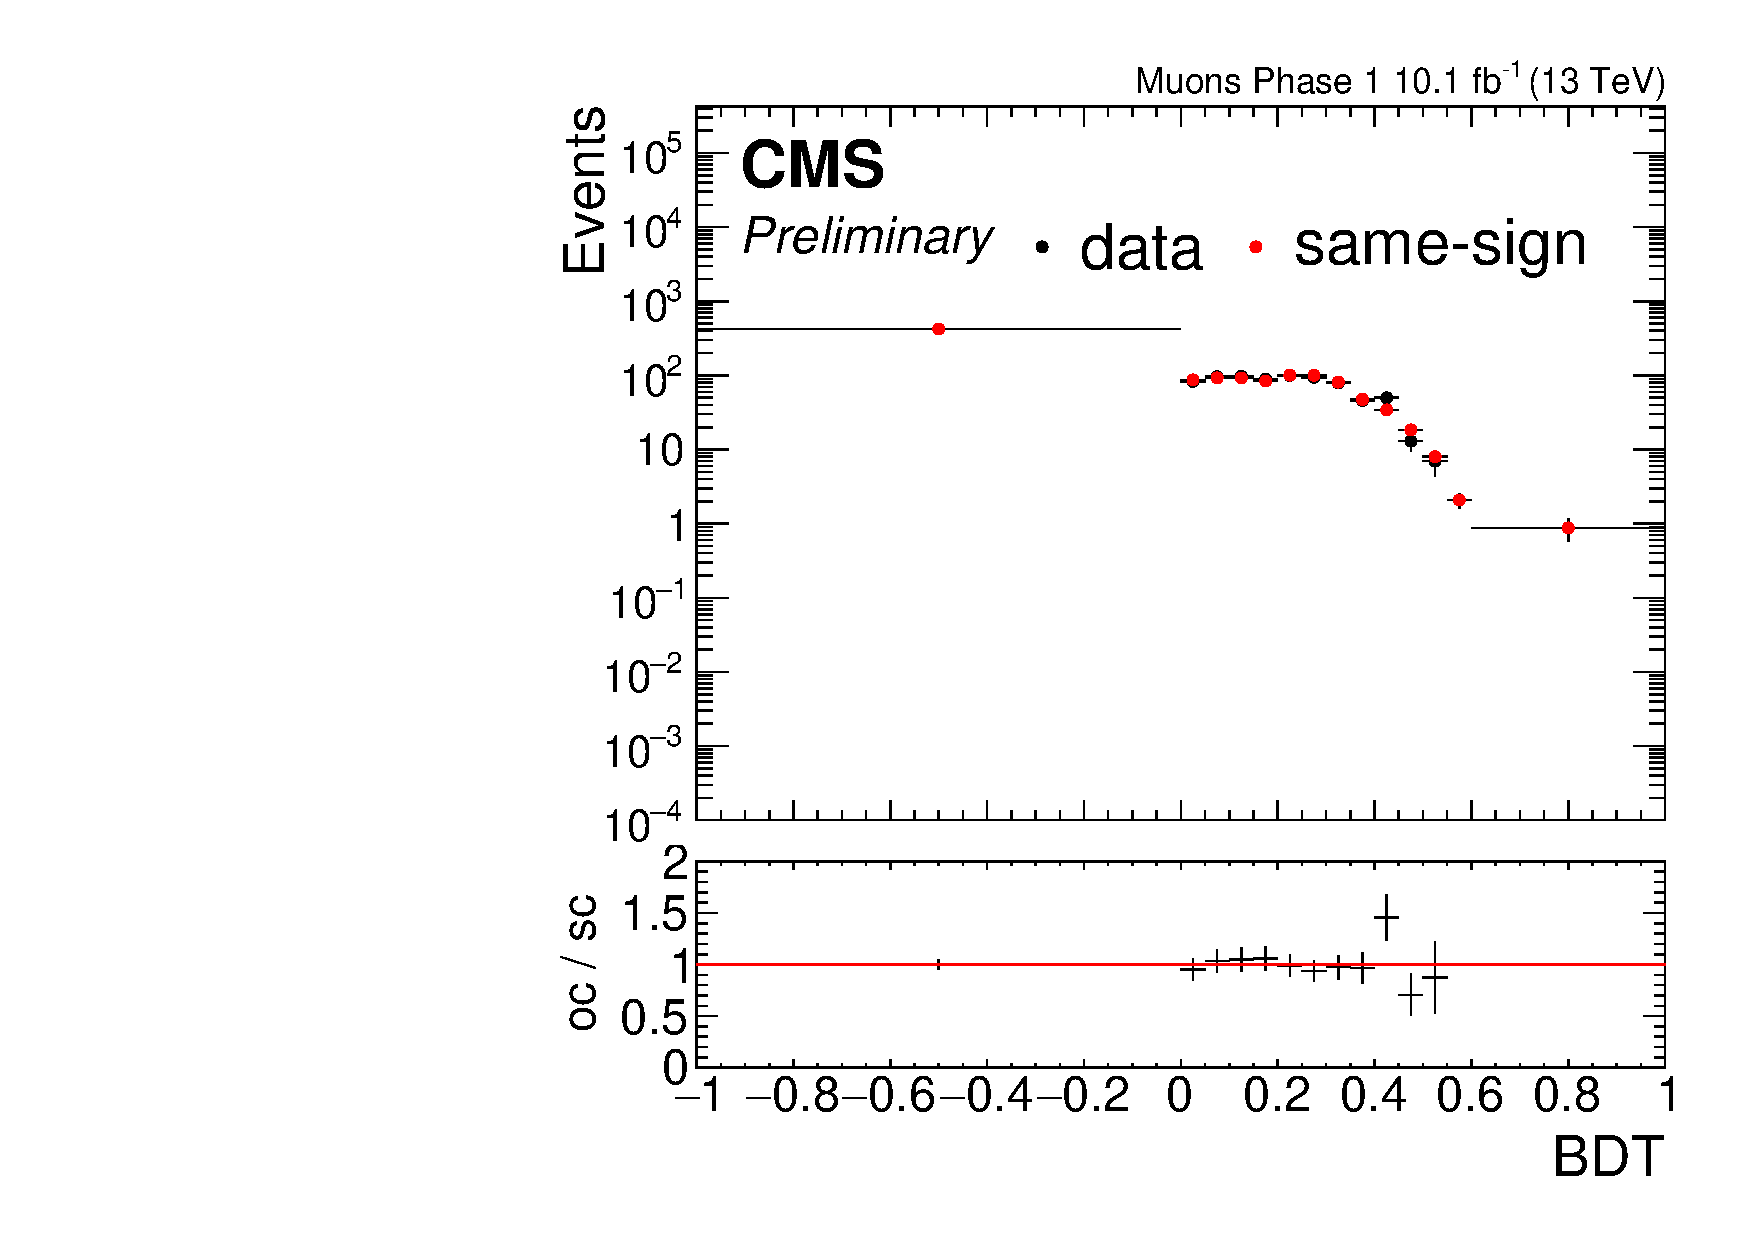
\includegraphics[width=0.48\linewidth]{plots/partial_unblinded_track_muon_sc_comparison_phase1/none_exTrack_dilepBDT_binsCorrJetNoMultIso10Dr0.6_log.pdf} \\

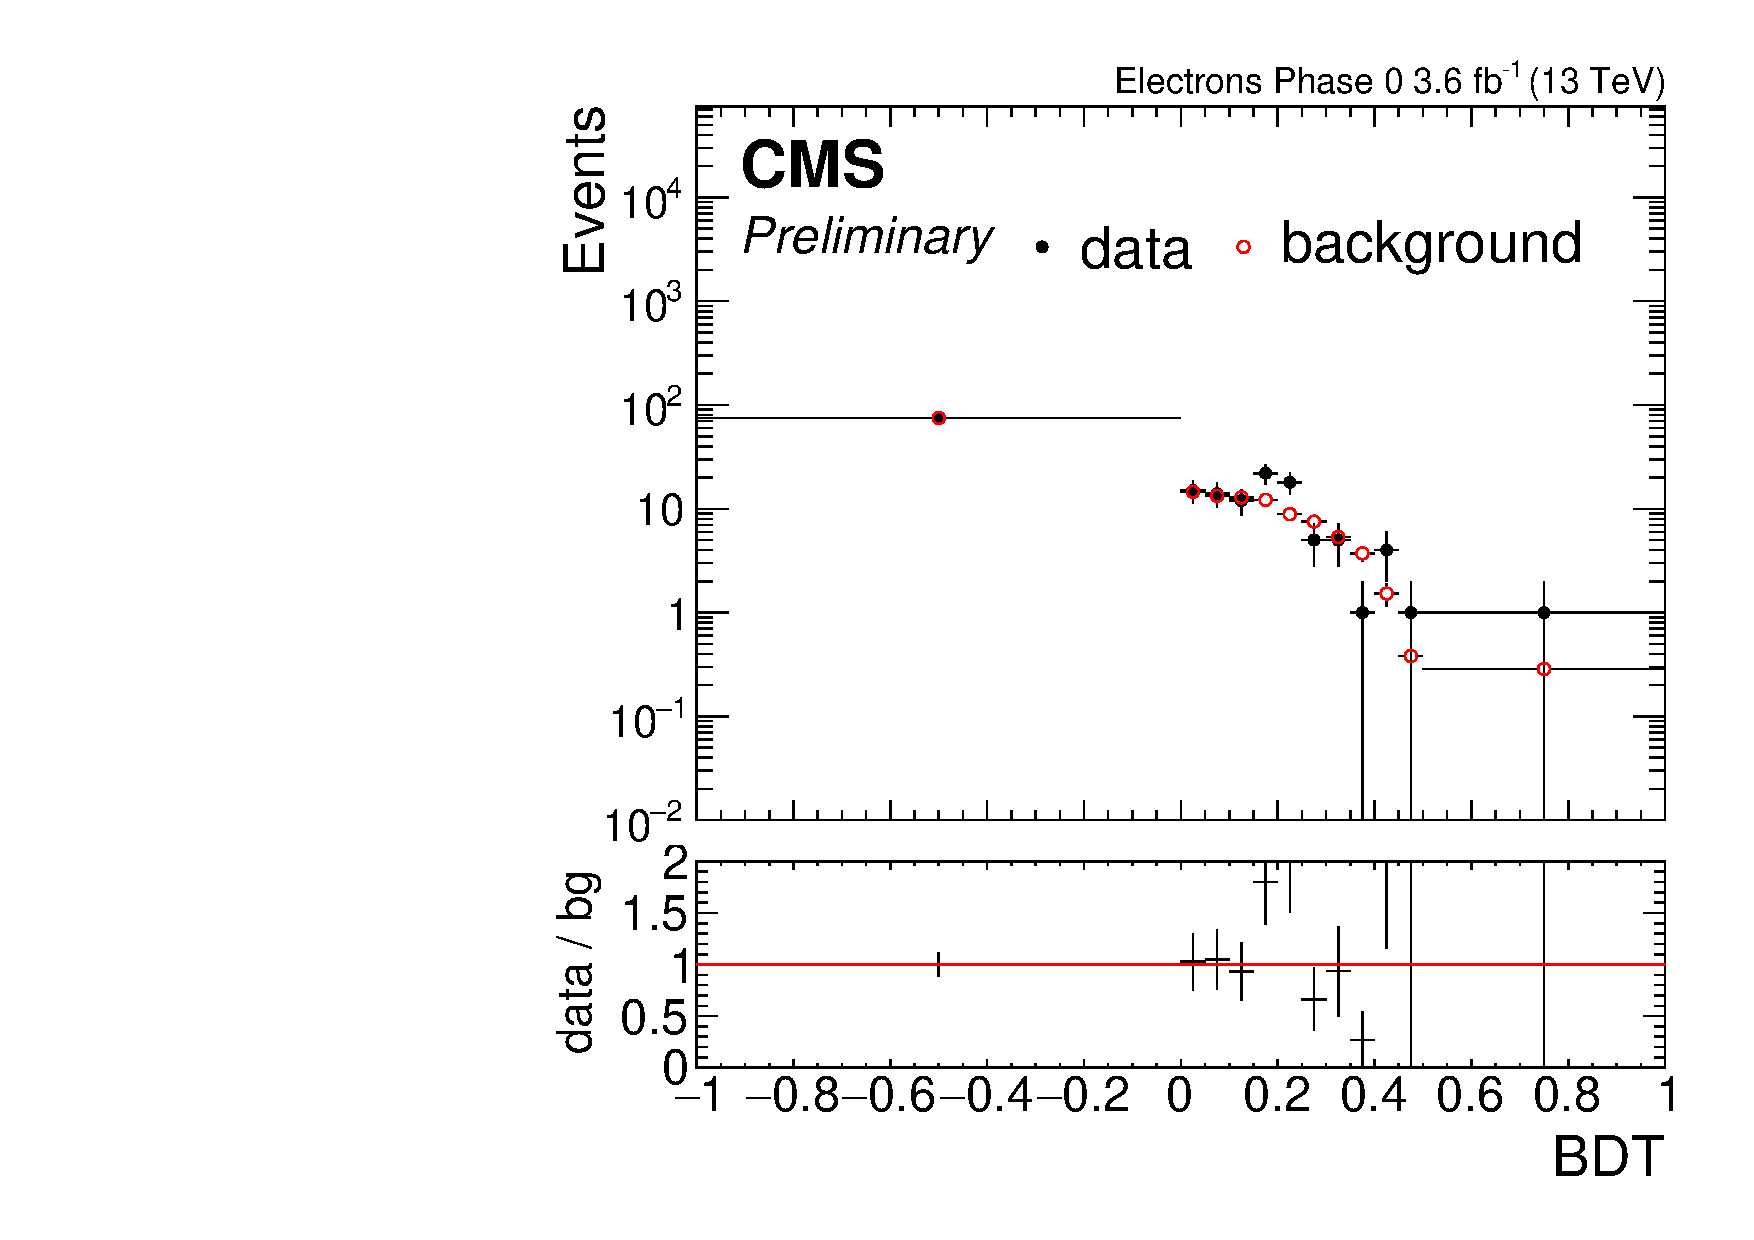
\includegraphics[width=0.48\linewidth]{plots/partial_unblinded_track_electrons_sc_comparison/none_exTrack_dilepBDT_binsCorrJetNoMultIso10Dr0.5_log.pdf} \,
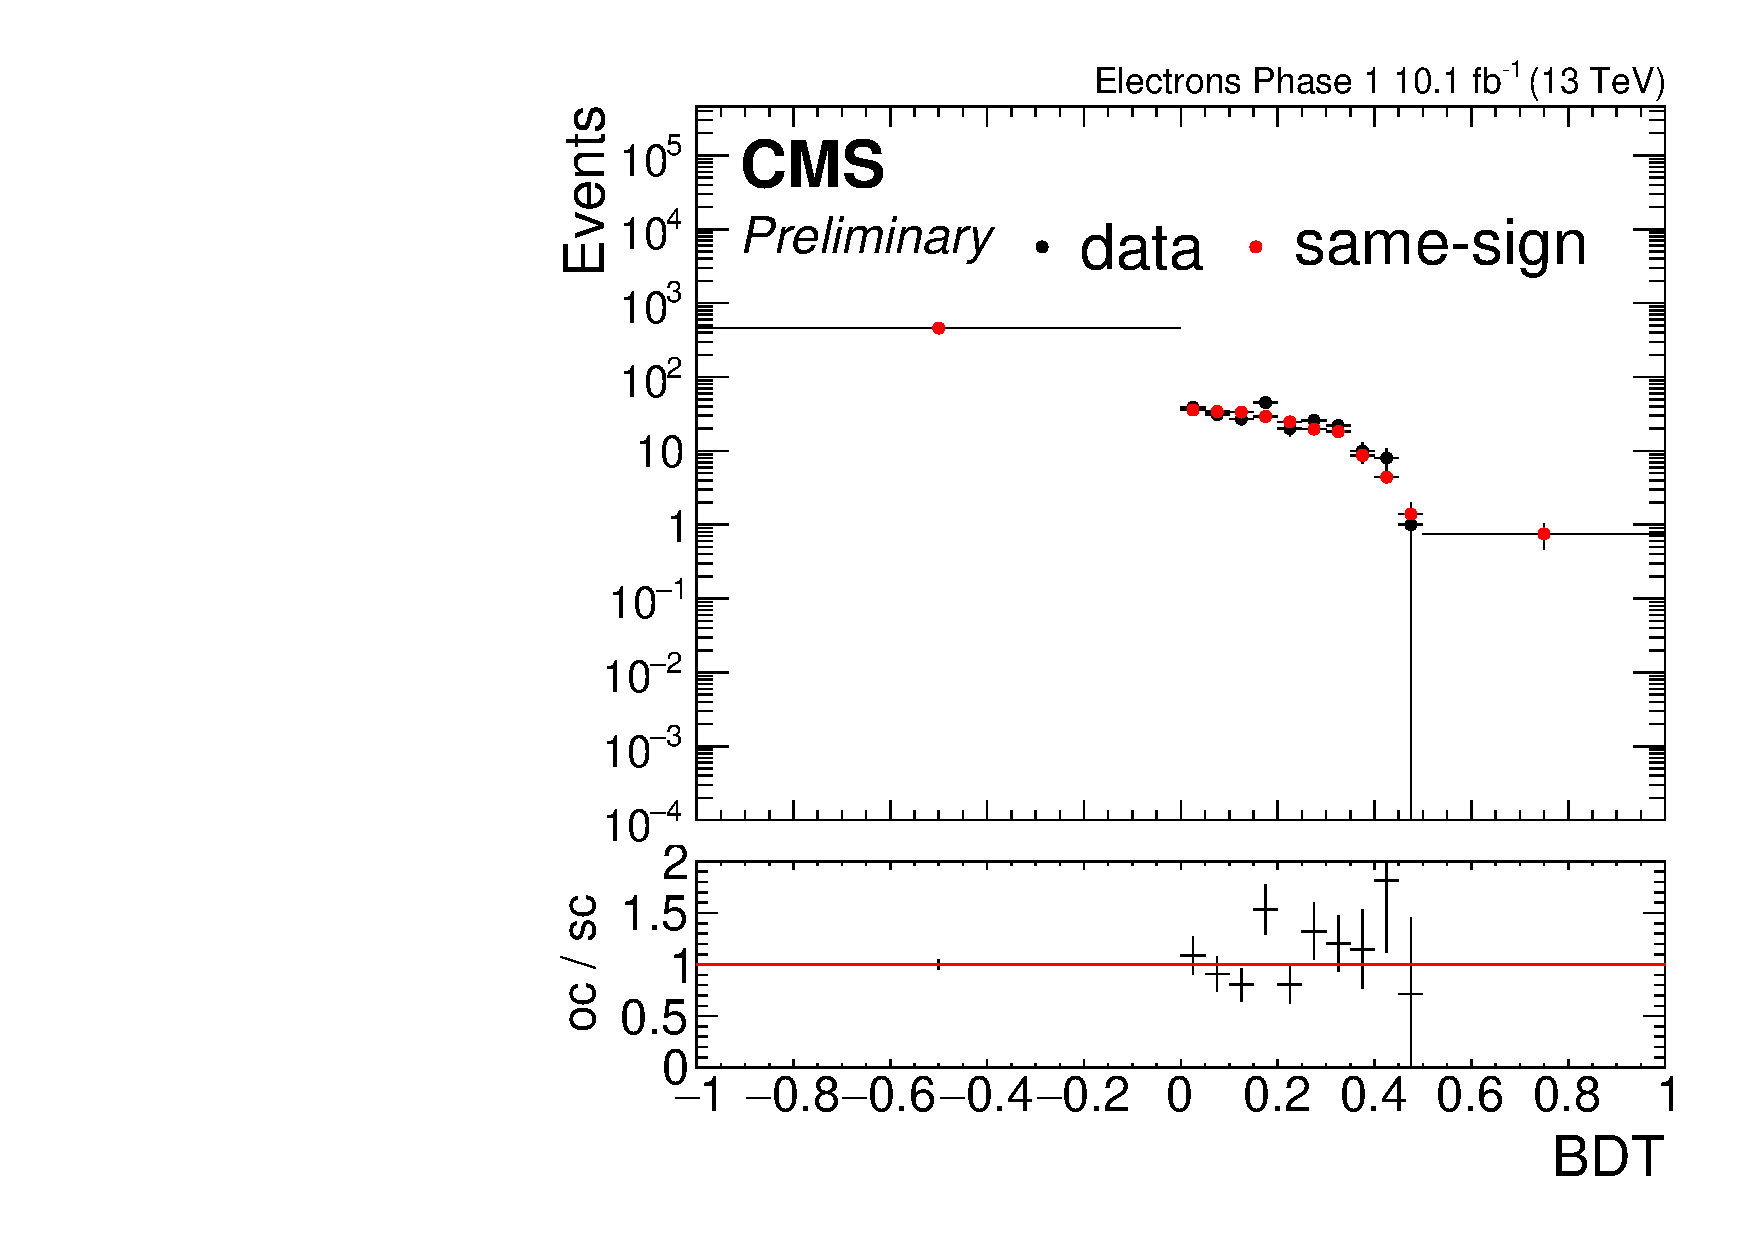
\includegraphics[width=0.48\linewidth]{plots/partial_unblinded_track_electrons_sc_comparison_phase1/none_exTrack_dilepBDT_binsCorrJetNoMultIso10Dr0.5_log.pdf} \\

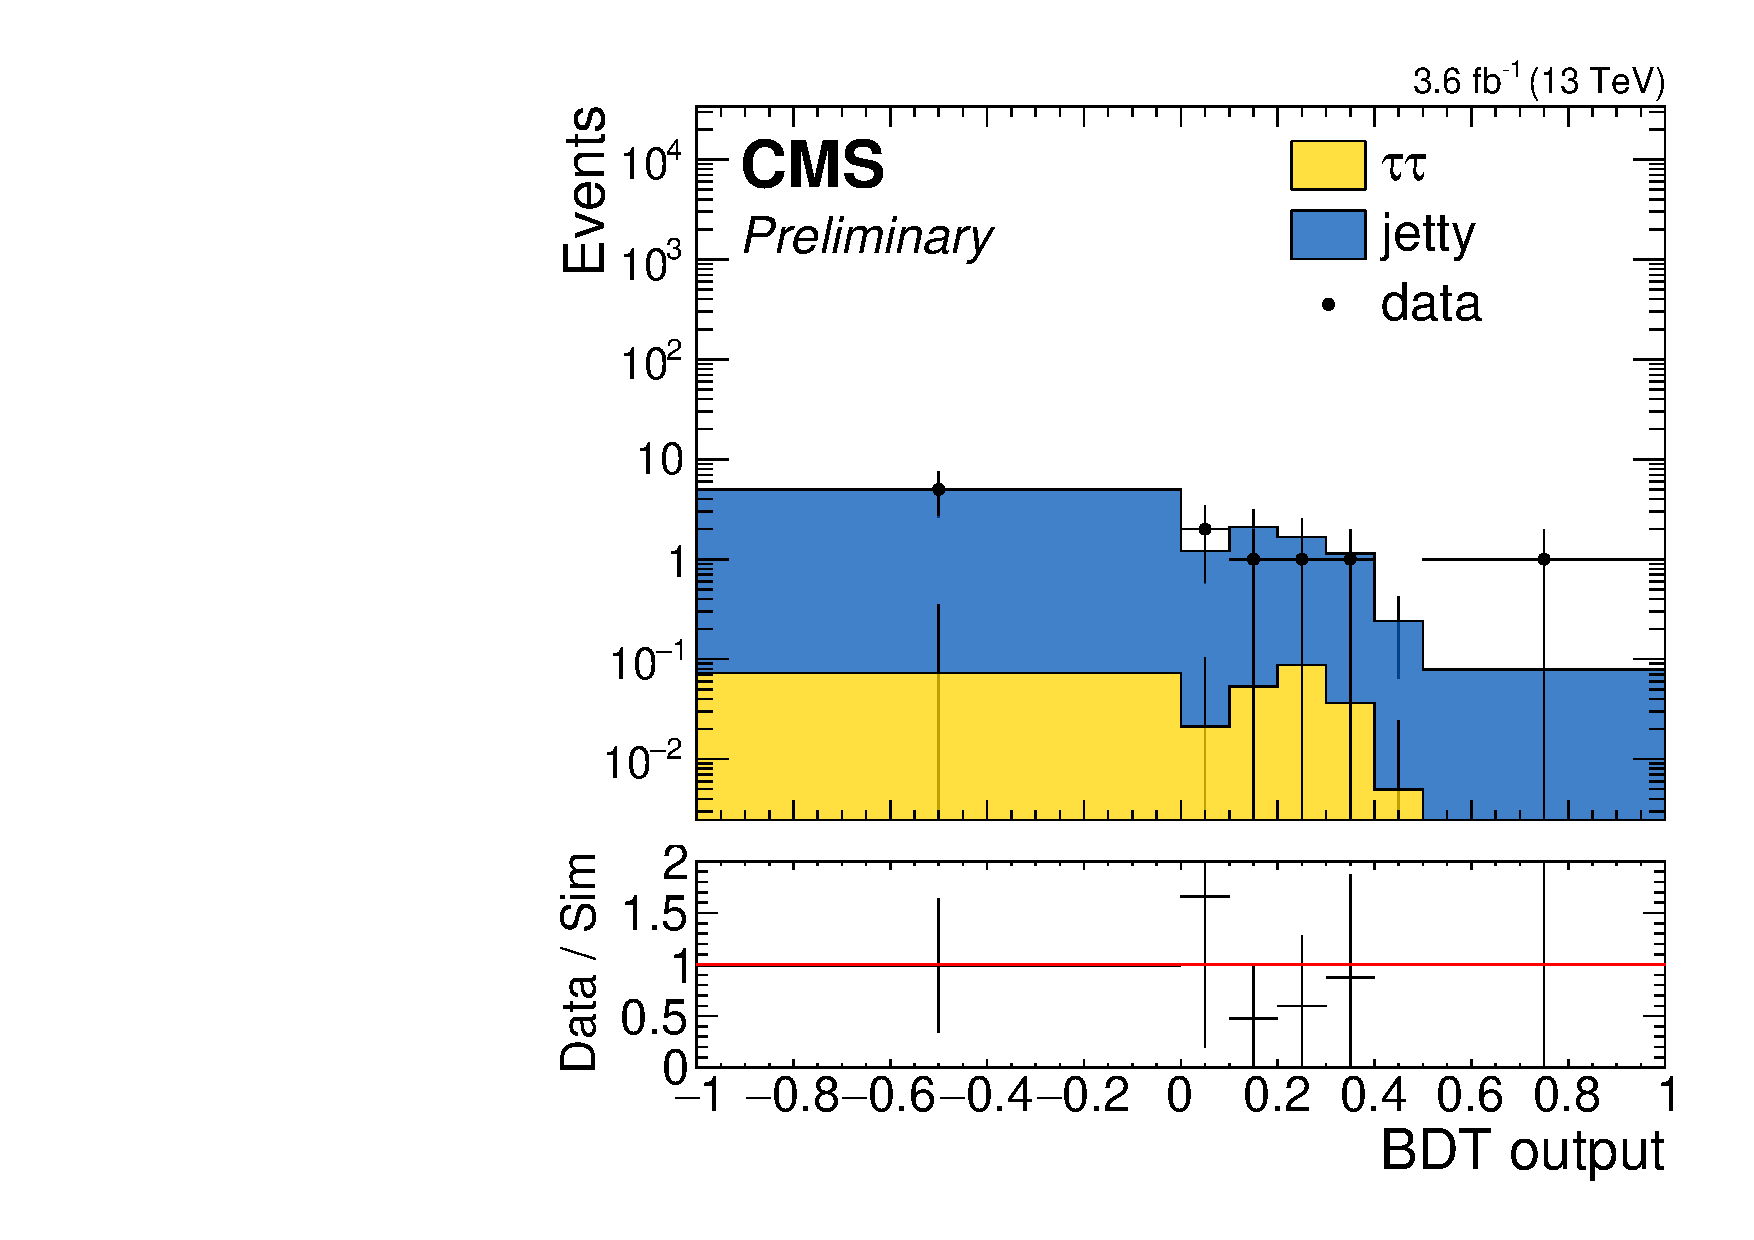
\includegraphics[width=0.48\linewidth]{plots/partial_unblinded_dimuon/sos_final_dilepBDTphase1CorrJetNoMultIso10Dr0.6_log.pdf} \,
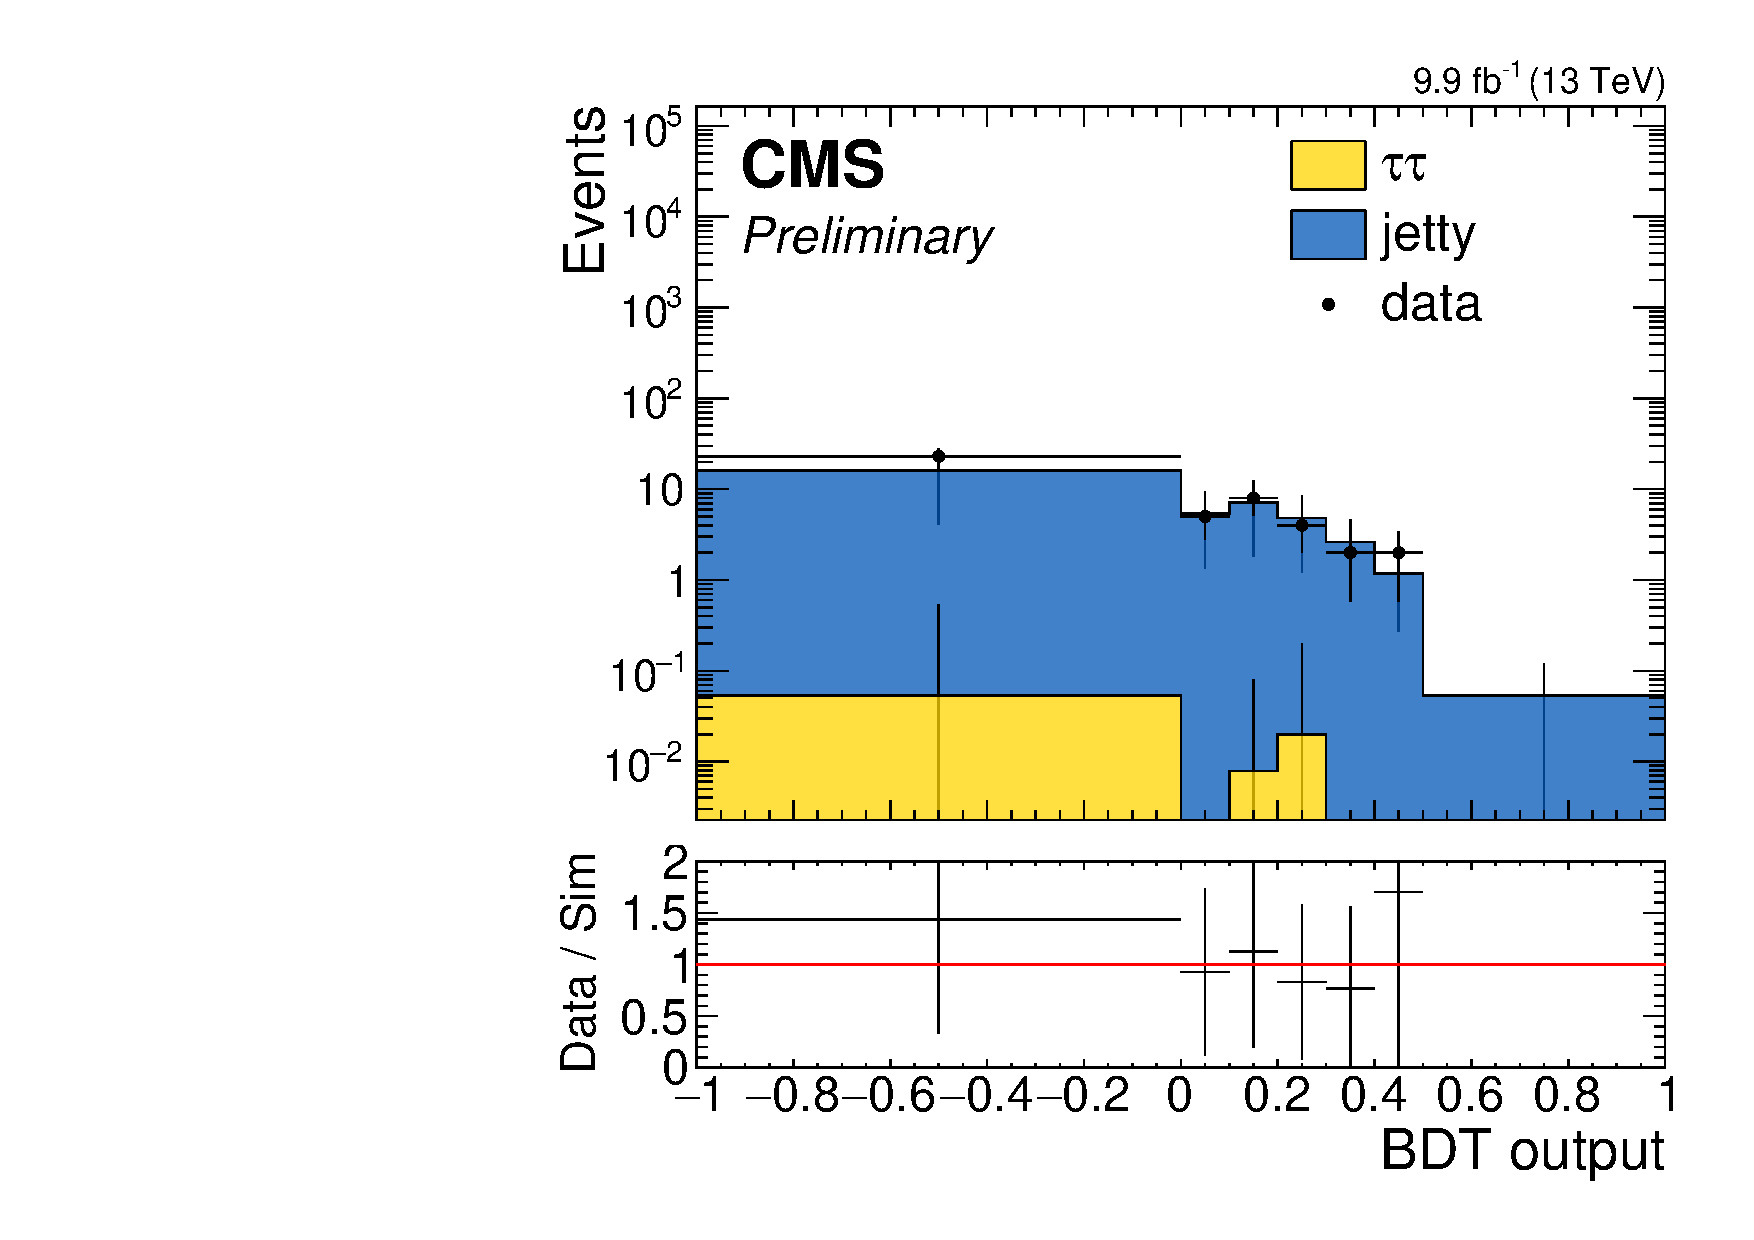
\includegraphics[width=0.48\linewidth]{plots/partial_unblinded_dimuon_phase1/sos_final_dilepBDTCorrJetNoMultIso10Dr0.6_log.pdf} \\

\caption[Partially unblinded results]{Partially unblinded results using 10\% of run 2 luminosity. Top row shows muon plus track for phase 0 (left) and phase 1 (right). Middle row shows electron plus track for phase 0 (left) and phase 1 (right). Bottom row shows the dimuon category for phase 0 (left) and phase 1 (right).}
\label{fig:unblinded_results}
\end{figure}

\begin{figure}[!htb]
\centering
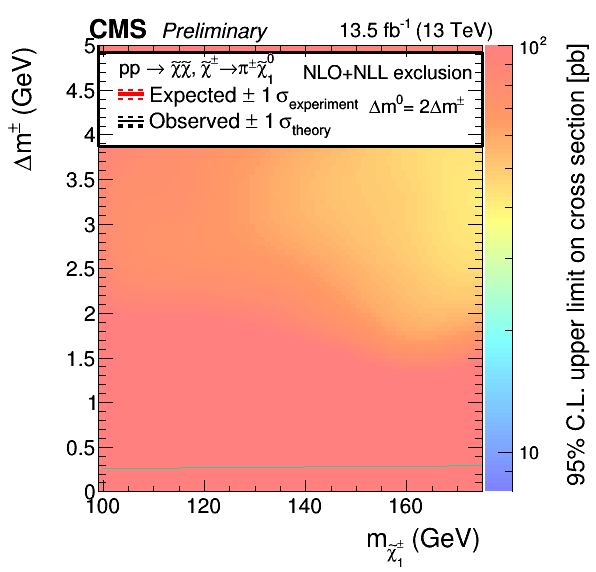
\includegraphics[width=0.48\linewidth]{plots/limits/observed/PureHiggsino_1tElectrons_ObservedXSEC.png} \,
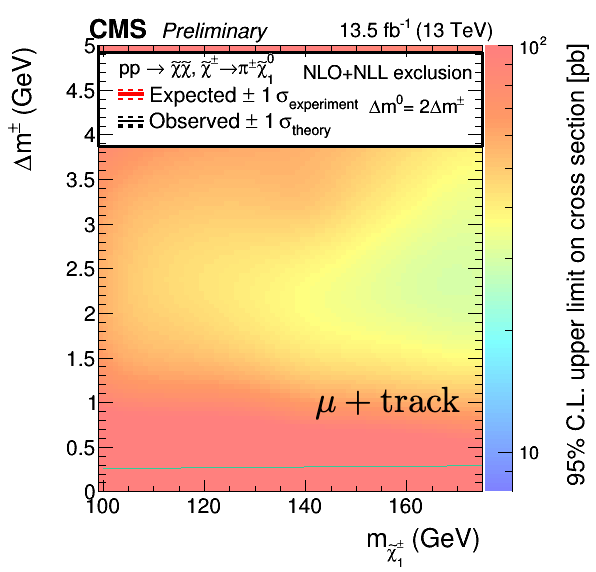
\includegraphics[width=0.48\linewidth]{plots/limits/observed/PureHiggsino_1tMuons_comb_ObservedXSEC.png} \\

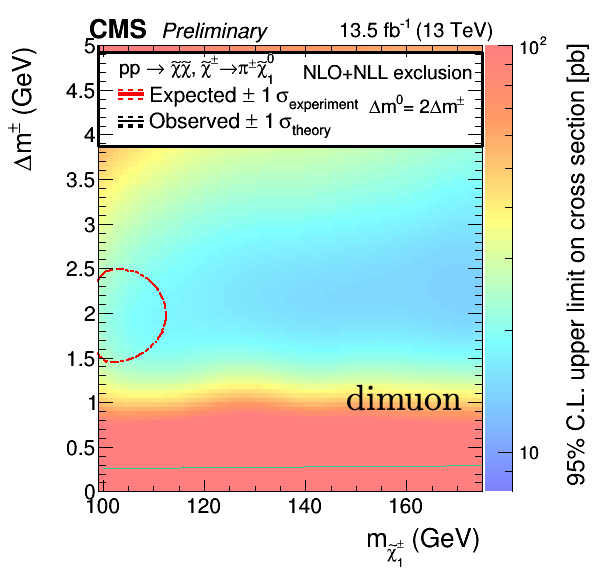
\includegraphics[width=0.48\linewidth]{plots/limits/observed/PureHiggsino_2lMuonsOrth_ObservedXSEC.png} \,
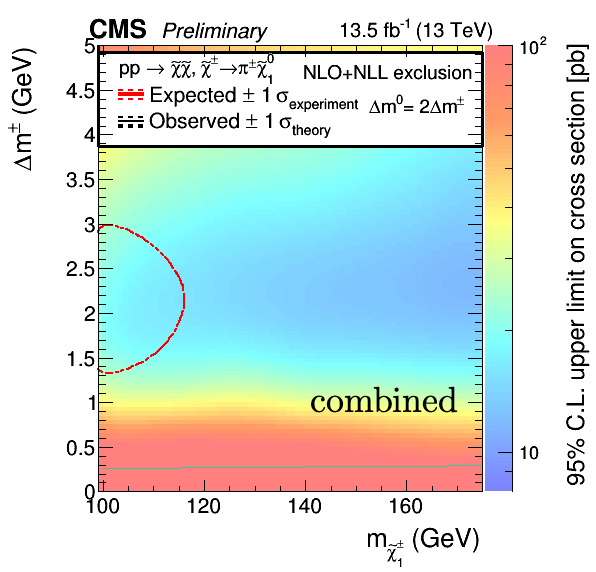
\includegraphics[width=0.48\linewidth]{plots/limits/observed/PureHiggsino_SoftPromptRun2_Observed_XSEC.png} \\

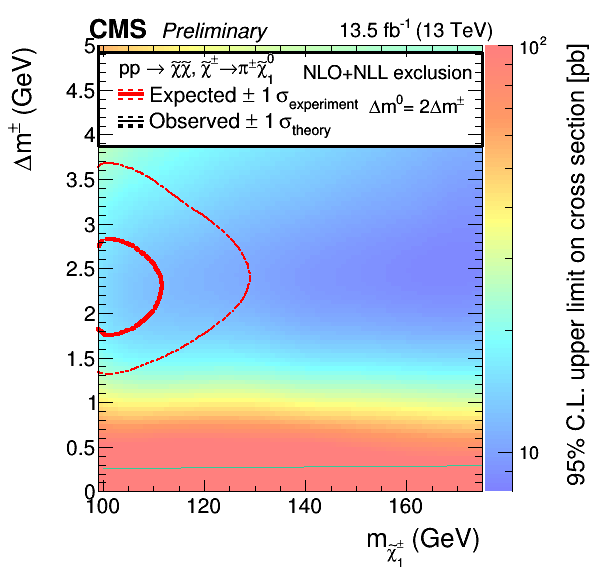
\includegraphics[width=0.48\linewidth]{plots/limits/observed/PureHiggsino_SoftPromptRun2Inc_ObservedXSEC.png} \\

\caption[Expected and observed limits for 10\% luminosity of run 2]{Expected and observed limits for 10\% luminosity of run 2. Top row shows limits for exclusive track plus electron (muon) on the left (right). The middle row shows limits for the dimuon category (left) and the combined limits for all categories (right). The bottom row shows the combined limits for all categories for the relaxed condition without SOS orthogonality.}
\label{fig:observed_limits}
\end{figure}
